% Author: Carles Marin (Claude, Anthropic, as AI research assistant).
% Part II. Which SU(4) representations contain the Standard-Model quark cell on T^2/Z_2:
% an exact criterion from a Levi branching and the orbifold chiral projection.
% Question-threaded narrative; honest about scope throughout. Build: pdflatex x2.
\documentclass[11pt,a4paper]{article}
\usepackage[utf8]{inputenc}
\usepackage{amsmath,amssymb,amsthm}
\usepackage{booktabs}
\usepackage[table,dvipsnames]{xcolor}
\usepackage{graphicx}
\usepackage{tikz}
\usetikzlibrary{shapes.geometric,arrows.meta,positioning,fit,backgrounds}
\usepackage{geometry}
\geometry{margin=2.4cm}
\usepackage[colorlinks=true,linkcolor=RoyalBlue,citecolor=BrickRed,urlcolor=RoyalBlue]{hyperref}
\usepackage{caption}
\captionsetup{font=small,labelfont=bf}
\newtheorem{theorem}{Theorem}
\newtheorem{lemma}{Lemma}
\newcommand{\ZZ}{\mathbb{Z}}
\newcommand{\RR}{\mathbb{R}}
\newcommand{\su}[1]{SU(#1)}
\definecolor{okgreen}{RGB}{0,140,54}
\definecolor{hdrblue}{RGB}{31,78,121}
\definecolor{softgrey}{RGB}{238,242,247}

\title{\textbf{Three Gates to a Quark Generation}\\[3pt]
\textbf{An Exact Criterion for Which $SU(4)$ Representations Contain the Standard Model,\\
and Why the Gauge Group Is Critical at Rank Three}\\[5pt]
\large\textnormal{Part II --- the $\pm\tfrac12$ cell, a Levi branching, and the orbifold
chiral projection}}
\author{Carles Mar\'in\thanks{Independent researcher, \texttt{karlesmarin@gmail.com}.
The computations were carried out and cross-checked with Claude (Anthropic) as an AI
research assistant against a common machine-verifiable ground truth (exact rational
arithmetic on $SU(n)$ weight systems in SageMath); every count in this paper regenerates
from the ancillary scripts.}}
\date{\today\\[2pt]\small DOI: \href{https://doi.org/10.5281/zenodo.21432628}{10.5281/zenodo.21432628}}

\begin{document}
\maketitle

\begin{abstract}
\noindent
The companion paper embedded a full Standard-Model quark generation in the
dimension-$60$ representation $(3,\mathbf{60})$ of $SU(4)$ on $T^2/\mathbb{Z}_2$ and
showed, by an exhaustive scan, that $(3,\mathbf{60})$ is the \emph{smallest} representation
able to do so. That minimality begs the general question: \emph{which} $SU(4)$
representations can hold a quark generation, and why only those? We answer it exactly. An
irreducible representation with Dynkin labels $(a,b,c)$ contains the Standard-Model quark
cell $\{Q(\mathbf{2},\tfrac16),\,u(\mathbf{1},\tfrac23),\,d(\mathbf{1},-\tfrac13)\}$ in its
$T^2/\mathbb{Z}_2$ chiral zero modes if and only if
\[
(a+2b+3c)\ \text{odd}\quad\wedge\quad b\ge 1\quad\wedge\quad a+b+c\ge 3 .
\]
The three clauses are, in order, an \emph{arithmetic} condition (the $\ZZ_4$ centre
charge), a \emph{geometric} one (the middle node of $SU(4)$ excited), and a \emph{size}
one (enough room to close the cell). We derive the criterion by deleting the middle node
of the $SU(4)$ Dynkin diagram --- exposing a Levi subgroup
$SU(2)_L\times SU(2)_R\times U(1)$ --- and projecting the resulting Clebsch--Gordan tower
onto the orbifold's chiral zero modes; the projection collapses the tower to a closed-form
zero-mode count $N=(b+1)(a+c+1)/2$. We are explicit about what is new and what is
inherited: the centre gate is classical, the branching is Littlewood--Richardson, and the
midpoint property (the doublet's $\tfrac16$ is the mean of the singlets' $\tfrac23$ and
$-\tfrac13$) reflects the Pati--Salam hypercharge relation; what is ours is the chiral
projection that yields the closed count, the packaged
criterion, and the reading of the cell as the invariant object. Finally we place $SU(4)$
in a family: the cell imposes three charge constraints on a hypercharge functional with
$\mathrm{rank}(G)-1$ free parameters, so it is a \emph{rigid} obstruction exactly at
$\mathrm{rank}=3$ --- $SU(4)$ is the marginal case, and for higher rank a generic
representation admits. The same counting explains, as a consumed-degree-of-freedom effect,
why a pinned hypercharge in higher-rank models leaves quarks with the wrong (integer)
charges and forces them onto a brane.
\end{abstract}

% ===================================================================
\section{From one representation to all of them}\label{sec:intro}
This paper continues a story its companion began. Part~I~\cite{PartI} took up a question
open since 2003, when Scrucca, Serone, Silvestrini and Wulzer observed that on an orbifold
the vanishing of localized tadpoles and the cancellation of anomalies are \emph{independent}
requirements, and named the missing piece --- an anomaly-free spectrum with a globally
vanishing tadpole --- as an open problem~\cite{SSSW}. Part~I met it in the six-dimensional
two-Higgs-doublet $SU(4)$ model of Akamatsu, Hirose, Maru and Nago~\cite{AHMN}: it embedded
a colored quark block in the dimension-$60$ representation $(3,\mathbf{60})$, exhibited a
$45$-multiplet completion cancelling anomalies and tadpole together, and proved an
\emph{Existence theorem} --- on that fermion library the tadpole never obstructs an
anomaly-free completion --- turning a computational witness into a structural guarantee. It
closed with a proposal: wherever a model-building result reads ``we found one,'' ask whether
the find was in fact a law. This paper takes Part~I at its word. For in passing, and without
explaining why, Part~I had recorded a second find --- an exhaustive scan showing
$(3,\mathbf{60})$ to be the \emph{smallest} $SU(4)$ representation able to host a full quark
generation. Why that one, and why so few? We turn the scanned fact into an exact law.

That question is older than the model, and its history is one of boxes packed ever tighter.
A grand-unified or gauge--Higgs construction begins by choosing a representation to carry the
matter, and the choice is severely constrained: the representation must contain, among its
states, exactly the quantum numbers of one generation. Georgi and Glashow fit a generation
into the $\overline{\mathbf 5}\oplus\mathbf{10}$ of $SU(5)$~\cite{GeorgiGlashow} --- in two
pieces, and with no seat for a right-handed neutrino. A year later the $\mathbf{16}$ spinor
of $SO(10)$ closed the box: fifteen Standard-Model fermions, and a sixteenth place the spinor
simply \emph{has}, all but forcing one to seat a $\nu_R$ there~\cite{SO10FM,SO10G} --- the
group knowing, as it were, before we did. The exceptional $\mathbf{27}$ of $E_6$ followed,
volunteering a generation plus exotics~\cite{E6}, and Georgi asked outright for all three
families in one irreducible representation~\cite{GeorgiFlavor,Yamatsu}, a dream that founders on a
hall of mirror fermions. Through all of it Slansky's tables were the field's phone-book for
deciding what a representation contains~\cite{Slansky}; the recent census of Herms and
Ruhdorfer turns the tallies into a statistic --- what fraction of anomaly-free matter is
unifiable~\cite{HermsRuhdorfer}. But the decision stayed, representation by representation, a
lookup rather than a law.

A minimum is an invitation. If one representation is smallest, there is a landscape behind
it --- and Part~I mapped a single point of it. What distinguishes the representations that
succeed from those that fail? Is ``$(3,\mathbf{60})$'' an accident of dimension, or the
first member of a family with a clean rule? This paper gives the rule, exactly, and reads
off from it why the family is so sparse, why the minimum falls where it does, and why the
gauge group is $SU(4)$ and not something larger. Where Part~I validated a witness, Part~II
charts the space around it; together they run from one consistent model to an understanding
of the whole matter landscape it lives in.

The organizing object throughout is what we will call the \emph{Standard-Model cell}: the
color-triplet quark content of one generation, stripped to its electroweak skeleton,
\[
Q\,(\mathbf{2},\tfrac16),\qquad u\,(\mathbf{1},\tfrac23),\qquad d\,(\mathbf{1},-\tfrac13).
\]
The up and down singlets are the doublet displaced in hypercharge by $\pm\tfrac12$ --- the
right-handed isospin $T^3_R$ of the Pati--Salam relation we meet in \S\ref{sec:cell}. The
operative fact is a small piece of arithmetic: the doublet's $\tfrac16$ is the \emph{mean}
of the singlets' charges, $\tfrac16=\tfrac12\!\big(\tfrac23+(-\tfrac13)\big)$, so the
doublet sits at the exact hypercharge midpoint of its two singlets. That midpoint is what
makes the cell a rigid geometric object in the weight lattice, and it is where our criterion
begins.

\paragraph{Scope and relation to prior work.} We are careful to separate what is new from
what is inherited, and most of the ingredients are inherited. The centre-charge gate ---
that admitting the Standard Model's fractional hypercharges forces a fixed congruence class
of the gauge-group centre --- is classical, stated for the Standard Model's own $\ZZ_6$ by
Hucks and by Saller and revisited by Tong and by Alonso, Dimakou and
West~\cite{Hucks,Saller,Tong,Alonso}. The branching we use is a maximal-parabolic Levi
restriction, whose multiplicities are Littlewood--Richardson coefficients~\cite{Fulton,GW}.
The midpoint relation is the Pati--Salam hypercharge identity, and the observation that a
hypercharge functional embedded in a simple group has a fixed number of free parameters is
the same counting that underlies the classic ``$\mathrm{rank}\ge 4$'' lower bound on
unified groups; a closely related Cartan-functional analysis of gauge-Higgs models, though
of the gauge-boson sector rather than the matter cell, is due to Aranda and
Wudka~\cite{ArandaWudka}. We claim no new group theory. What is ours is threefold:
(i) the \emph{exact three-gate criterion} for $SU(4)$ on $T^2/\mathbb{Z}_2$, packaged as a
single closed statement (\S\ref{sec:theorem}); (ii) the \emph{orbifold chiral projection}
that collapses the Levi Clebsch--Gordan tower to the closed-form zero-mode count
$N=(b+1)(a+c+1)/2$ (\S\ref{sec:levi}); and (iii) the reading of the $\pm\tfrac12$ cell as
the invariant, together with the placement of $SU(4)$ at the critical rank
(\S\ref{sec:rank}) --- the last an interpretive lens on classical ingredients, not a new
theorem. Figure~\ref{fig:roadmap} is the route.

\begin{figure}[t]
\centering
\resizebox{\textwidth}{!}{%
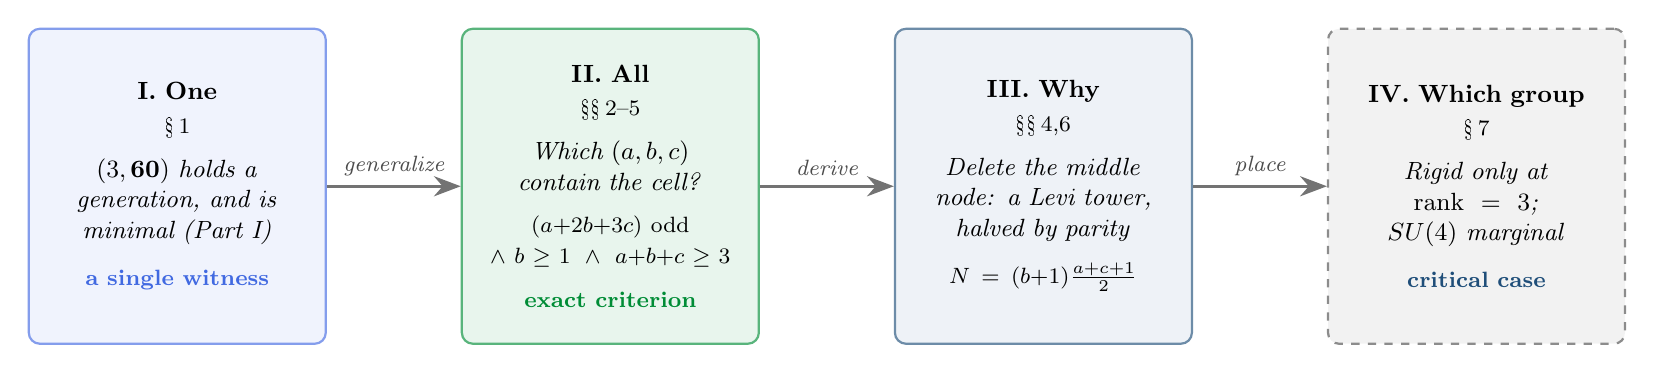
\begin{tikzpicture}[font=\small,
  act/.style={rounded corners,draw,thick,text width=3.35cm,align=center,inner sep=6pt,minimum height=4.0cm,anchor=north},
  arr/.style={-{Stealth[length=3.4mm]},very thick,black!55}]
\node[act,fill=RoyalBlue!8,draw=RoyalBlue!65] (a1) at (0,0)
 {\textbf{I.\ One}\\[1pt]{\footnotesize\S\,1}\\[5pt]
  \textit{$(3,\mathbf{60})$ holds a}\\\textit{generation, and is}\\\textit{minimal (Part I)}\\[6pt]
  {\footnotesize\color{RoyalBlue}\textbf{a single witness}}};
\node[act,fill=okgreen!9,draw=okgreen!65] (a2) at (5.5,0)
 {\textbf{II.\ All}\\[1pt]{\footnotesize\S\S\,2--5}\\[5pt]
  \textit{Which $(a,b,c)$}\\\textit{contain the cell?}\\[6pt]
  {\footnotesize$(a{+}2b{+}3c)$ odd\\$\wedge\ b\ge1\ \wedge\ a{+}b{+}c\ge3$}\\[5pt]
  {\footnotesize\color{okgreen}\textbf{exact criterion}}};
\node[act,fill=softgrey,draw=hdrblue!65] (a3) at (11.0,0)
 {\textbf{III.\ Why}\\[1pt]{\footnotesize\S\S\,4,6}\\[5pt]
  \textit{Delete the middle}\\\textit{node: a Levi tower,}\\\textit{halved by parity}\\[6pt]
  {\footnotesize $N=(b{+}1)\tfrac{a+c+1}{2}$}};
\node[act,fill=black!5,draw=black!45,dashed] (a4) at (16.5,0)
 {\textbf{IV.\ Which group}\\[1pt]{\footnotesize\S\,7}\\[5pt]
  \textit{Rigid only at}\\\textit{$\mathrm{rank}=3$;}\\\textit{$SU(4)$ marginal}\\[6pt]
  {\footnotesize\color{hdrblue}\textbf{critical case}}};
\draw[arr] (a1.east) -- node[above,font=\footnotesize\itshape,black!70]{generalize} (a2.west);
\draw[arr] (a2.east) -- node[above,font=\footnotesize\itshape,black!70]{derive} (a3.west);
\draw[arr] (a3.east) -- node[above,font=\footnotesize\itshape,black!70]{place} (a4.west);
\end{tikzpicture}}
\caption{The route of this paper. From the single minimal witness of Part I to an exact
criterion for all representations; the criterion is derived by a Levi branching and a
chiral projection, and $SU(4)$ is then placed as the unique marginal rank at which the
cell is a rigid obstruction.}
\label{fig:roadmap}
\end{figure}

% ===================================================================
\section{The Standard-Model cell as a lattice problem}\label{sec:cell}
What does it mean, exactly, for a representation to \emph{contain} the Standard Model ---
and can we decide it by a calculation rather than a search through states? To make the
question sharp we first strip a generation to the object that must be present.
Colour plays no active role in what follows: in the model of Part I the strong $SU(3)_c$
is a spectator factor and the quark block is $(\mathbf 3, R)$ with $R$ a representation of
$SU(4)$, so ``colour triplet'' is automatic and the electroweak content lives entirely in
$R$. The weak $SU(2)_L$ is generated by the first simple root of $SU(4)$, and the
hypercharge is a Cartan direction commuting with it. Writing a weight of $SU(4)$ in the
partition coordinates $(n_1,n_2,n_3,n_4)$ and the two independent $SU(2)_L$-invariant
charges
\[
q_8=n_1+n_2-2n_3,\qquad q_{15}=n_1+n_2+n_3-3n_4,
\]
the unbroken hypercharge that reproduces the Standard-Model quark charges is
$Y=(-7q_8+4q_{15})/18$~\cite{PartI}, a specific element of the two-parameter family of
traceless $SU(2)_L$-invariant functionals $Y=\alpha q_8+\beta q_{15}$.

A representation \emph{contains the cell} if its zero modes include a left-handed weak
doublet $Q$ and two right-handed weak singlets $u,d$ whose charges under a single such
$Y$ are $\tfrac16,\tfrac23,-\tfrac13$. Because $Y$ is linear and homogeneous, this is an
exact linear-algebra condition. Collecting the charge vectors of the three multiplets,
the cell closes precisely when
\begin{equation}\label{eq:det}
\det\!\begin{pmatrix} q_8^{Q} & q_{15}^{Q} & \tfrac16\\[2pt]
q_8^{u} & q_{15}^{u} & \tfrac23\\[2pt] q_8^{d} & q_{15}^{d} & -\tfrac13\end{pmatrix}=0
\qquad\text{with the top $2\times2$ minor nonzero,}
\end{equation}
i.e.\ the target vector $(\tfrac16,\tfrac23,-\tfrac13)$ lies in the span of the two charge
columns, so a unique $Y$ pins all three values. Equation~\eqref{eq:det} turns ``contains
the Standard Model'' into a statement about the affine geometry of the weight diagram.

One consequence is immediate and organizing. Since
$\tfrac16=\tfrac12\big(\tfrac23+(-\tfrac13)\big)$,
the doublet charge is the \emph{mean} of the two singlet charges; if the doublet sits at
the midpoint $Q=\tfrac12(u+d)$ of the singlets in charge space, then $Y(Q)=\tfrac16$ holds
\emph{automatically} once $Y(u)=\tfrac23$ and $Y(d)=-\tfrac13$. The cell is a symmetric
$\pm\tfrac12$ reflection pair straddling the doublet --- the geometric face of the
half-century-old Pati--Salam hypercharge relation $Y=T^3_R+(B-L)/2$~\cite{PatiSalam} (with
$Q_{\rm em}=T^3+Y$, so $T^3_R=0$ for the doublet and $\pm\tfrac12$ for the singlets, and
$B-L=\tfrac13$ for a quark); the very $\pm\tfrac12$ that names the cell is Pati and Salam's
right-handed isospin.\footnote{A caution against a natural pun: the group carrying our cell
is the electroweak $SU(4)$ of the AHMN model, with colour a \emph{separate} $SU(3)_c$; it is
not the colour $SU(4)_c$ of Pati and Salam, in which lepton number is a fourth colour. What
we borrow from~\cite{PatiSalam} is the hypercharge relation, not the group.} The whole
problem is now: for which $(a,b,c)$
does the weight diagram of $R$ offer such a configuration among its parity-selected zero
modes?

\emph{Established here:} containing the Standard Model reduces to an exact rank
condition~\eqref{eq:det} on the weight diagram, with the $\pm\tfrac12$ cell a symmetric
reflection pair. \emph{Left open:} which labels $(a,b,c)$ actually offer that
configuration --- the three gates of the rest of the paper.

% ===================================================================
\section{The centre gate (classical)}\label{sec:centre}
Before asking \emph{where} the charges sit, a blunter question: which representations can
display the Standard-Model fractions $\tfrac16,\tfrac23,\tfrac13$ \emph{at all}? The first
obstruction is arithmetic and is not ours. The value of a hypercharge on a
weight is, up to normalization, an integer combination of the labels divided by the order
of the centre; the Standard-Model fractions $\tfrac16,\tfrac23,\tfrac13$ can be reached
only from a fixed congruence class. For $SU(4)$ the relevant invariant is the $\ZZ_4$
centre charge, equal to the $n$-ality
\begin{equation}
c(R)=a+2b+3c \pmod 4,
\end{equation}
Slansky's congruency class~\cite{Slansky}. A direct check on the hypercharge above shows
the quark fractions occur only when this class is \emph{odd}. That fractional hypercharge
is locked to the centre charge in exactly this way is a classical fact, stated for the
Standard Model's own $\ZZ_6=\ZZ_2\times\ZZ_3$ by Hucks and by Saller, and recast in
one-form / global-structure language by Tong and by Alonso, Dimakou and
West~\cite{Hucks,Saller,Tong,Alonso}. We claim none of it; we record that, transferred to
the $\ZZ_4$ centre of the embedding group, it is the first of our three clauses.

\emph{Established here:} gate one, $(a+2b+3c)$ odd, is the classical centre-charge
congruence, inherited not invented. \emph{Left open:} the two geometric gates, which the
weight diagram --- not the centre --- must supply.

% ===================================================================
\section{Delete the middle node: the Levi tower and its chiral projection}\label{sec:levi}
The centre says the fractions are reachable. But reachable \emph{together}, under one
hypercharge --- and where, in $SU(4)$ itself, is that decided? The remaining two clauses,
and the reason for them, come from a single structural move.
The Dynkin diagram of $SU(4)$ is a path of three nodes,
$\circ\!-\!\circ\!-\!\circ$; \emph{deleting the middle node} splits it into two disjoint
$SU(2)$'s and leaves one $U(1)$:
\begin{equation}
SU(4)\ \supset\ \underbrace{SU(2)_L}_{\text{node }\alpha_1}\ \times\
\underbrace{SU(2)_R}_{\text{node }\alpha_3}\ \times\ \underbrace{U(1)_m}_{\text{deleted }\alpha_2}.
\end{equation}
$SU(2)_L$ is the weak isospin. The deleted node carries the $U(1)$ charge
\begin{equation}
m\ :=\ 2q_8+q_{15}\ =\ 3(n_1+n_2-n_3-n_4),
\end{equation}
which --- as one checks on the simple roots --- is changed only by the middle root
$\alpha_2$ and left fixed by $\alpha_1,\alpha_3$: it is the coordinate conjugate to the
middle node. This single observation controls both remaining gates.

Branch an irreducible $(a,b,c)$ to this Levi. Its $SU(2)_L$-\emph{singlet} sector --- the
seat of the right-handed quark singlets $u,d$ --- has a clean shape
(Figure~\ref{fig:levi}, verified on all representations to dimension $700$): it consists of
\begin{equation}\label{eq:tower}
(b+1)\ \text{copies of the Clebsch--Gordan tower}\quad
[\tfrac a2]\otimes[\tfrac c2]\ =\ \bigoplus_{j=|a-c|/2}^{(a+c)/2}[j],
\end{equation}
one copy at each of $b+1$ equally spaced values of $m$ (spacing $12$, so the singlets span
a middle-node extent of exactly $12b$). The number of copies is set by the middle label
$b$; the internal $SU(2)_R$ spin content is set by the outer labels $a,c$, with
\emph{maximal} spin $(a+c)/2$.

Now impose the orbifold. On $T^2/\mathbb{Z}_2$ the two $\ZZ_2$ parities assign chirality;
on the singlet sector they are locked (one is redundant), so the surviving right-handed
zero modes are exactly \emph{half} of each tower, and --- because the distinct hypercharges
are set by the tower's \emph{extent}, i.e.\ its top spin $(a+c)/2$ --- the count of distinct
right-handed colour-singlet charge slots is
\begin{equation}\label{eq:count}
\boxed{\,N(a,b,c)\ =\ (b+1)\cdot\frac{a+c+1}{2}\,}
\end{equation}
(the outer factor is an integer because $a+c$ is odd whenever the centre charge is odd).
Equation~\eqref{eq:count} is the technical heart of the paper: a closed-form count of
chiral zero-mode multiplets as a function of the bulk representation's Dynkin labels. The
count factorizes as
\[
N=\underbrace{(b+1)(a+c+1)}_{\text{Levi branching (dimension-independent)}}\ \times\ \underbrace{\tfrac12}_{\text{orbifold projection}},
\]
a form that makes the roles transparent: the group theory is inherited (a
Littlewood--Richardson evaluation~\cite{Fulton,GW}), while the halving is the
extra-dimensional projection. It is the \emph{extremal chiral projection} --- keep the top
spin, halve by parity --- that is ours, not the closed form it produces.

\emph{Established here:} a closed chiral zero-mode count $N=(b+1)(a+c+1)/2$, with
middle-node extent $12b$, from one Levi branching and the parity projection. \emph{Left
open:} how this count decides whether the cell closes --- the criterion of
\S\ref{sec:theorem}.

\begin{figure}[t]
\centering
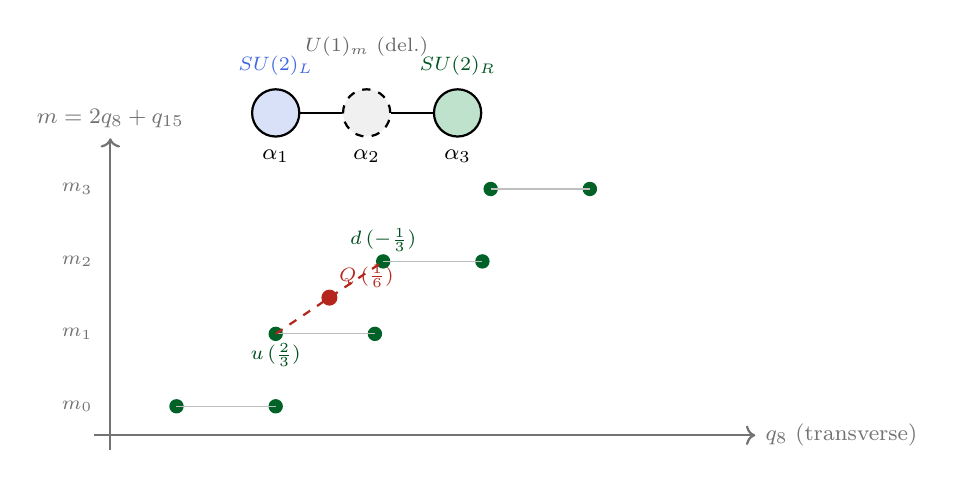
\begin{tikzpicture}[font=\small,x=1.05cm,y=0.92cm]
% Dynkin diagram, middle node deleted (placed in a clear band above the lattice)
\begin{scope}[shift={(1.6,4.25)}]
  \node[circle,draw,thick,fill=RoyalBlue!20,minimum size=6mm] (d1) at (0,0){};
  \node[circle,draw,thick,dashed,fill=black!6,minimum size=6mm] (d2) at (1.1,0){};
  \node[circle,draw,thick,fill=okgreen!25,minimum size=6mm] (d3) at (2.2,0){};
  \draw[thick] (d1)--(d2)--(d3);
  \node[below=1pt of d1,font=\footnotesize]{$\alpha_1$};
  \node[below=1pt of d2,font=\footnotesize]{$\alpha_2$};
  \node[below=1pt of d3,font=\footnotesize]{$\alpha_3$};
  \node[above=1pt of d1,font=\scriptsize,RoyalBlue]{$SU(2)_L$};
  \node[above=8pt of d2,font=\scriptsize,black!60]{$U(1)_m$ (del.)};
  \node[above=1pt of d3,font=\scriptsize,okgreen!60!black]{$SU(2)_R$};
\end{scope}
% the sheared lattice for (0,3,3): b+1=4 levels in m, (a+c+1)/2=... show schematic
\draw[->,black!55,thick] (-0.6,-0.2) -- (7.4,-0.2) node[right,font=\footnotesize]{$q_8$ (transverse)};
\draw[->,black!55,thick] (-0.4,-0.4) -- (-0.4,3.9) node[above,font=\footnotesize]{$m=2q_8+q_{15}$};
\foreach \lev/\yy in {0/0.2, 1/1.2, 2/2.2, 3/3.2}{
  \node[left,font=\scriptsize,black!55] at (-0.5,\yy){$m_\lev$};
}
% level points, sheared right as m increases; two points per level (RH kept), extremal in q8
\foreach \yy/\xa/\xb in {0.2/0.4/1.6, 1.2/1.6/2.8, 2.2/2.9/4.1, 3.2/4.2/5.4}{
  \fill[okgreen!70!black] (\xa,\yy) circle (2.6pt);
  \fill[okgreen!70!black] (\xb,\yy) circle (2.6pt);
  \draw[black!25] (\xa,\yy)--(\xb,\yy);
}
% mark a symmetric cell: doublet Q at midpoint of u,d across two levels
\fill[BrickRed] (2.25,1.7) circle (2.9pt);
\node[BrickRed,font=\scriptsize,above right] at (2.25,1.7){$Q\,(\tfrac16)$};
\node[okgreen!55!black,font=\scriptsize,below] at (1.6,1.2){$u\,(\tfrac23)$};
\node[okgreen!55!black,font=\scriptsize,above] at (2.9,2.2){$d\,(-\tfrac13)$};
\draw[BrickRed,dashed,thick] (1.6,1.2)--(2.9,2.2);
\end{tikzpicture}
\caption{Deleting the middle node of $SU(4)$ exposes $SU(2)_L\times SU(2)_R\times U(1)_m$.
The right-handed colour-singlet zero modes (green) form a sheared lattice: $b+1$ levels in
the middle-node charge $m$ (here $b=3$, four levels), each carrying half of a
Clebsch--Gordan tower. A Standard-Model cell (red/green, dashed) is a symmetric
$\pm\tfrac12$ pair $u,d$ whose midpoint is a weak doublet $Q$ at hypercharge $\tfrac16$.
The cell can close only when the lattice is genuinely two-dimensional --- which needs the
middle node excited ($b\ge1$) and at least three singlets ($a+b+c\ge3$).}
\label{fig:levi}
\end{figure}

% ===================================================================
\section{The cell criterion}\label{sec:theorem}
We now hold an exact count of the singlets; when is a count enough to close a cell? The
count~\eqref{eq:count} decides the last two gates. The cell~\eqref{eq:det} needs a
\emph{two-dimensional} singlet lattice: three non-collinear charge slots, so that some
symmetric pair has a doublet at its midpoint. Reading this off the tower:
\begin{itemize}
\item if $b=0$ there is a single value of $m$: all singlets are collinear, and no
hypercharge can separate the cell. Hence $b\ge1$ is necessary --- the middle node must be
excited to open the transverse (spin-$SU(2)_R$) direction; the extent is exactly $12b$.
\item with $b\ge1$, the number of distinct singlets is $N=(b+1)(a+c+1)/2$; this drops to
$N=2$ only at the single corner $b=1,\ a+c=1$, i.e.\ $a+b+c=2$, where the two available
singlets are collinear and the cell is over-constrained. For every other case $N\ge3$ and
the lattice is two-dimensional. Hence $a+b+c\ge3$.
\end{itemize}
Together with the centre gate this gives the criterion, which we have verified exhaustively
against the direct construction~\eqref{eq:det} on all representations to dimension $900$.

\begin{theorem}[Cell criterion]\label{thm:cell}
A finite-dimensional irreducible representation $(a,b,c)$ of $SU(4)$ contains a full
Standard-Model quark cell $\{Q(\mathbf 2,\tfrac16),u(\mathbf 1,\tfrac23),d(\mathbf 1,-\tfrac13)\}$
among its right/left-handed $T^2/\mathbb{Z}_2$ chiral zero modes if and only if
\[
\boxed{\;(a+2b+3c)\ \text{is odd}\quad\wedge\quad b\ge1\quad\wedge\quad a+b+c\ge3\;}
\]
Equivalently: the centre charge is odd (arithmetic), the middle node is excited so the
right-handed colour-singlet lattice spreads over $12b$ in the middle-node charge
(geometric), and the lattice carries at least three non-collinear points
$N=(b+1)(a+c+1)/2\ge3$ (size).
\end{theorem}

\textbf{Theorem~\ref{thm:cell} is the central result of this paper, and the criterion is
ours}: the closed three-gate statement, and the chiral-projection count~\eqref{eq:count}
that produces it, are new. We say so without overclaiming --- Table~\ref{tab:gates} records
the three clauses and, beside each, exactly what is inherited from classical group theory
and what is new, so ownership is explicit gate by gate. The criterion is sparse: up to
dimension $400$ only eight representations
qualify (up to conjugation), of dimensions
$60,84,140,140,216,224,280,360$, and the smallest, $(a,b,c)=(0,2,1)$ of dimension $60$, is
precisely the $(3,\mathbf{60})$ of Part I --- so Theorem~\ref{thm:cell} recovers, and
explains, the minimality found there by brute force.

\emph{Established here:} the exact criterion (Theorem~\ref{thm:cell}), which recovers the
minimality of Part~I as its smallest instance. \emph{Left open:} why $SU(4)$, of all
groups, makes the cell a rigid gate at all --- the subject of \S\ref{sec:rank}.

\begin{table}[t]
\centering\small
\begin{tabular}{p{3.4cm}p{4.9cm}p{5.4cm}}
\toprule
\rowcolor{hdrblue}
\textcolor{white}{Gate} & \textcolor{white}{Inherited (cite)} & \textcolor{white}{Ours}\\
\midrule
$(a{+}2b{+}3c)$ odd\newline\emph{(arithmetic)} &
$\ZZ_4$ centre / $n$-ality congruence; fractional $Y$ locked to the
centre~\cite{Hucks,Saller,Tong,Alonso,Slansky} &
transfer to the $\ZZ_4$ of the embedding group as gate 1 of a single closed criterion\\
\midrule
\rowcolor{softgrey}
$b\ge1$\newline\emph{(geometric)} &
Levi branching / Clebsch--Gordan tower~\cite{Fulton,GW} &
the middle-node extent $=12b$; its necessity for a chiral doublet at $Y=\tfrac16$\\
\midrule
$a+b+c\ge3$\newline\emph{(size)} &
--- &
the closed chiral zero-mode count $N=(b{+}1)(a{+}c{+}1)/2$ and its
$N\ge3$ threshold\\
\bottomrule
\end{tabular}
\caption{The three gates of Theorem~\ref{thm:cell}, and an honest ledger of what each owes
to classical group theory and what is new here. The novelty is the chiral projection giving
the closed count, and the packaging of all three into one criterion --- not the centre
arithmetic nor the branching.}
\label{tab:gates}
\end{table}

\begin{figure}[t]
\centering
\includegraphics[width=0.86\linewidth]{fig_cell_landscape.pdf}
\caption{The admissibility landscape of Theorem~\ref{thm:cell}, over the label plane
$(a+c,\,b)$ (the centre gate restricts to $a+c$ odd). The background is the exact zero-mode
count $N=(b+1)(a+c+1)/2$; a green ring marks a representation passing all three gates, a red
cross one that fails. The gates carve the admissible region cleanly: the whole $b=0$ row
falls (middle node not excited), as does the single corner $a+c=1,\,b=1$ (too small,
$N=2$). The minimum, $(0,2,1)=\mathbf{60}$ of Part~I, sits at the lower-left corner of the
admissible region. Every marker is computed, not schematic.}
\label{fig:landscape}
\end{figure}

\begin{figure}[t]
\centering
\includegraphics[width=0.80\linewidth]{fig_cell_lattice.pdf}
\caption{The right-handed colour-singlet weight lattice of a concrete admissible
representation, $(0,3,3)$, computed exactly. The singlets (filled, coloured by the
middle-node charge $m=2q_8+q_{15}$) form the sheared $(b{+}1)\times\frac{a+c+1}{2}$ lattice
of \S\ref{sec:levi} --- here four $m$-levels ($b=3$). Faint grey squares are the weak
doublets. A Standard-Model cell (red) is a symmetric $\pm\tfrac12$ pair $u,d$ whose midpoint
is a doublet $Q$; the shear is exactly what lets three points fail to be collinear, so the
cell can close. This is the data behind the schematic of Figure~\ref{fig:levi}.}
\label{fig:latticereal}
\end{figure}

% ===================================================================
\section{An aside on node-independence}\label{sec:nodeindep}
Why is that count so clean --- is $(a{+}1)(b{+}1)(c{+}1)$ an accident of $SU(4)$, or does
the group insist on it? The clean shape of~\eqref{eq:count} rests on a small general fact worth isolating, if only
to see where $SU(4)$'s tidiness ends. For a simple root $\alpha$, write
$\dim\mathrm{Inv}_\alpha(V)$ for the dimension of the subspace of a representation $V$
annihilated by the $SU(2)$ generated by $\alpha$.

\begin{lemma}\label{lem:node}
For any irreducible representation of a simple Lie algebra, $\dim\mathrm{Inv}_\alpha(V)$
depends only on the Weyl orbit --- equivalently the length --- of the simple root $\alpha$.
In a simply-laced algebra (all roots one length, hence one Weyl orbit) it is therefore
independent of which simple root is chosen; in a non-simply-laced algebra it takes at most
two values, one for long and one for short roots.
\end{lemma}

\begin{proof}
Weight multiplicities are Weyl-invariant. For $w$ in the Weyl group,
$\langle w\mu,(w\alpha)^\vee\rangle=\langle\mu,\alpha^\vee\rangle$, so the distribution of
$\alpha$-eigenvalues over the (Weyl-stable) weight multiset is the same for $\alpha$ and
$w\alpha$; hence so is $\dim\mathrm{Inv}_\alpha=N_\alpha(0)-N_\alpha(2)$. In a simply-laced
algebra all roots lie in one Weyl orbit.
\end{proof}

For $SU(4)$ (type $A_3$, simply-laced) the invariant dimension is thus the same at every
node, and equals the clean product $(a+1)(b+1)(c+1)$. This product form, however, is
special to $A_3$: it is the linear factor of the $A_3$ Weyl dimension polynomial, and it
fails already for $SU(5)$, where the node-independent value is a Littlewood--Richardson sum
with no such factorization (for instance it takes the prime value $11$ at labels
$(1,1,0,0)$, which no product of linear factors reproduces across the lattice). We verified
Lemma~\ref{lem:node} on types $A_2\!-\!A_4,\,D_4$ (node-independent) and
$B_2,B_3,C_3,G_2,F_4$ (two values, split exactly by long/short root, e.g.\ $F_4$ giving
$[21,21,15,15]$). The lemma is elementary and likely folklore; we include it because it
identifies precisely which of $SU(4)$'s coincidences is generic (node-independence) and
which is exceptional (the product), and the latter is one of several senses in which
$SU(4)$ is special --- the subject of the next section.

% ===================================================================
\section{Why $SU(4)$? The critical rank}\label{sec:rank}
Is the criterion a statement about the Standard Model, or about $SU(4)$? Enlarge the group,
and the answer separates the two. Theorem~\ref{thm:cell} is about $SU(4)$; whether the same
rigidity survives for larger groups sharpens what ``$SU(4)$'' is really doing.
The cell imposes three charge constraints, $Y(Q)=\tfrac16$, $Y(u)=\tfrac23$,
$Y(d)=-\tfrac13$, on a hypercharge functional that, being traceless and
$SU(2)_L$-invariant, has $\mathrm{rank}(G)-1$ free parameters. The count is the whole story:
\begin{center}\small
\begin{tabular}{lccl}
\toprule
\rowcolor{hdrblue}
\textcolor{white}{group} & \textcolor{white}{rank} & \textcolor{white}{$Y$ parameters} &
\textcolor{white}{the cell}\\
\midrule
\rowcolor{softgrey}
$\boldsymbol{SU(4)}$ & $\mathbf 3$ & $\mathbf 2$ &
\textcolor{BrickRed}{\textbf{over-determined}} --- rigid arithmetic gate\\
$SU(5)$ & $4$ & $3$ & \textcolor{okgreen}{\textbf{marginally solvable}} --- gate dissolves\\
\rowcolor{softgrey}
$SU(6)$ & $5$ & $4$ & \textcolor{RoyalBlue}{\textbf{under-determined}} --- generic reps admit\\
\bottomrule
\end{tabular}
\end{center}
With three constraints and $\mathrm{rank}(G)-1$ parameters, the cell is a genuine
obstruction (a measure-zero alignment) exactly when $\mathrm{rank}(G)-1<3$, i.e.\ at
$\mathrm{rank}=3$. Among simple groups large enough to contain the cell, $SU(4)$ is the
unique marginal case; at rank $4$ and above a \emph{generic} anomaly-free representation
admits, the only residual obstruction being too few surviving modes. We have checked this
directly: with a free hypercharge, $73\%$ of $SU(5)$ and $85\%$ of $SU(6)$ representations
(to dimension $200$) admit, across all centre classes, whereas $SU(4)$ stays sparse and
centre-selective. The ``rank $\ge$ something'' arithmetic is classical; what the cell adds
is the reading that $SU(4)$ sits exactly at its margin.

\begin{figure}[t]
\centering
\includegraphics[width=0.68\linewidth]{fig_cell_dissolution.pdf}
\caption{The rigid cell gate dissolves above the critical rank. With a free hypercharge
functional ($\mathrm{rank}(G)-1$ parameters against three constraints), $SU(4)$ (rank $3$)
is over-determined and admits only a sparse, centre-selective set; $SU(5)$ and $SU(6)$
(rank $\ge4$) become generically solvable, and a large fraction of representations admit
across \emph{all} centre classes (measured to dimension $200$). The transition is the
counting of \S\ref{sec:rank}, not a property of any one group.}
\label{fig:dissolution}
\end{figure}

There is an honest caveat that is also the useful physics. ``Dissolves at higher rank''
assumes the hypercharge is \emph{free} to be any surviving combination. In a real model the
hypercharge is often \emph{pinned} --- fixed, say, by the requirement
$\sin^2\theta_W=\tfrac14$ that motivates these $SU(4)$ constructions. Pinning consumes the
free parameters, and then the obstruction can return at any rank. This is exactly what
happens in the recent $SU(7)$ grand gauge--Higgs model of Komori and Maru, where the bulk
hypercharge generator, fixed to reproduce $\sin^2\theta_W$, assigns only integer and
half-integer charges, ``so the fractional hypercharges of quarks cannot be obtained from
the [bulk] fields'' and the quarks are forced onto a brane~\cite{KomoriMaru}. Our counting
reads their integer/half-integer fact as a consumed-degree-of-freedom result: with the
hypercharge pinned, no residual Cartan freedom remains to place the fractional cell on bulk
colour triplets. The robust half of the story is the one that does not depend on the
assumption: $SU(4)$ is rigid \emph{even under maximal hypercharge freedom}, and that is why
its cell criterion is as sharp as Theorem~\ref{thm:cell}.

\emph{Established here:} $SU(4)$ is the unique rank at which the cell is a rigid
obstruction under a free hypercharge, and the same counting explains the higher-rank
bulk-quark obstruction as a consumed-freedom effect. \emph{Left open:} the precise
$\ZZ_N$-orbifold and general-$n$ dependence, laid out next.

% ===================================================================
\section{Reflections and proposals}\label{sec:reflections}
Three threads seem worth pulling.

\paragraph{The cell is the invariant.} Across the groups above, the gauge algebra, the
representation, the dimension and the centre all change; the $\pm\tfrac12$ cell does not. It
is the weak-isospin skeleton of one generation, the same object in every embedding, and the
criterion is best read not as ``which representations of $SU(4)$'' but as ``does the group
contain the cell in the correct centre sector, with room to close it.'' The centre supplies
the arithmetic, the geometry supplies the room; the cell supplies the target.

\paragraph{Dimension is a second knob.} The count factorizes as (Levi branching) $\times$
(orbifold projection). The first factor is dimension-independent; the second is where the
compactification enters. A single $\ZZ_2$ acting on the chirality axis halves the modes; a
$\ZZ_2$ locked to an existing axis --- as the second $T^2/\mathbb{Z}_2$ parity is on the
singlet sector, so that five- and six-dimensional counts here coincide --- does not; a
$\ZZ_N$ orbifold retains a fraction $1/N$. Higher-dimensional or higher-$N$ projections
therefore \emph{shrink} the mode count, so that the geometric-smallness obstruction (the
only one left at high gauge rank) can revive. Gauge rank and orbifold projection are
opposite knobs on the same cell: one dissolves the arithmetic gate, the other tightens the
geometric one. Making the $\ZZ_N$ dependence a precise counting theorem is a clean next step.

\paragraph{A closed form beyond $SU(4)$.} Lemma~\ref{lem:node} leaves open the exact
node-independent invariant dimension for $SU(n)$: it is a Littlewood--Richardson sum whose
$SU(4)$ specialization happens to be a product. Whether it admits a hook-content or
determinantal closed form --- and whether the ``triangular'' $SU(5)$ values
$\binom{k+2}{2}=\dim\mathrm{Sym}^k(\mathbb C^{3})$ generalize to
$\dim\mathrm{Sym}^k(\mathbb C^{n-2})$ for all symmetric powers --- is a well-posed
combinatorial question that our data already constrains.

% ===================================================================
\section{Conclusion}\label{sec:conclusion}
We have turned the minimality observed in Part I into an exact rule. An $SU(4)$
representation $(a,b,c)$ contains a Standard-Model quark cell on $T^2/\mathbb{Z}_2$ if and
only if its centre charge is odd, its middle node is excited, and its labels sum to at least
three; the derivation runs through a Levi branching whose Clebsch--Gordan tower, projected
onto the orbifold's chiral zero modes, yields the closed count $N=(b+1)(a+c+1)/2$. We have
been deliberate about credit: the centre arithmetic, the branching, and the
hypercharge-parameter counting are classical, and we cite them as such; what is ours is the
chiral projection that produces the closed count, the packaging into a single criterion, and
the reading of the $\pm\tfrac12$ cell as the invariant that places $SU(4)$ at the critical
rank. The last of these also explains, rather than merely restates, why higher-rank
constructions with a pinned hypercharge cannot keep their quarks in the bulk. The criterion
is exact and machine-checked; the questions it opens --- the general-$n$ closed form and
the $\ZZ_N$ dimension dependence --- are stated precisely enough to be settled. And it
closes back onto the thread Part~I left hanging: viability is decided model by model, but a
model must first be \emph{eligible}, and Theorem~\ref{thm:cell} is the eligibility test ---
it says which representations can even be entered into the search for a viable
six-dimensional $SU(4)$ generation. From one witness to the landscape it lives in, that is
the arc of the two papers.

\paragraph{Reproducibility.} Every count regenerates from the ancillary SageMath scripts:
the direct cell construction~\eqref{eq:det}, the Levi-branching derivation of~\eqref{eq:count},
the exhaustive criterion check to dimension $900$, the $SU(5)/SU(6)$ rank scans, and the
node-independence sweep across Lie types of Lemma~\ref{lem:node}.

\begin{thebibliography}{99}
\bibitem{PartI} C.~Mar\'in, \emph{Anomaly- and Tadpole-Compatible Fermion Completion of
Six-Dimensional $SU(4)$ Gauge--Higgs Unification} (Part~I), Zenodo (2026),
DOI:\,10.5281/zenodo.21432625.
\bibitem{SSSW} C.A.~Scrucca, M.~Serone, L.~Silvestrini, A.~Wulzer, \emph{Gauge-Higgs
Unification in Orbifold Models}, JHEP \textbf{02} (2004) 049, hep-th/0312267.
\bibitem{AHMN} K.~Akamatsu, T.~Hirose, N.~Maru, A.~Nago, \emph{Two Higgs Doublet Model from
Gauge--Higgs Unification in Six Dimensions}, arXiv:2603.05857; and
\emph{Gauge--Higgs Unification of $SU(4)$ Model}, arXiv:2312.08608.
\bibitem{PatiSalam} J.C.~Pati, A.~Salam, \emph{Lepton Number as the Fourth Color},
Phys.\ Rev.\ D \textbf{10} (1974) 275; Erratum \emph{ibid.} \textbf{11} (1975) 703.
\bibitem{GeorgiGlashow} H.~Georgi, S.L.~Glashow, \emph{Unity of All Elementary Particle
Forces}, Phys.\ Rev.\ Lett.\ \textbf{32} (1974) 438.
\bibitem{SO10FM} H.~Fritzsch, P.~Minkowski, \emph{Unified Interactions of Leptons and
Hadrons}, Ann.\ Phys.\ \textbf{93} (1975) 193.
\bibitem{SO10G} H.~Georgi, \emph{The State of the Art --- Gauge Theories}, in
\emph{Particles and Fields 1974}, AIP Conf.\ Proc.\ \textbf{23} (1975) 575.
\bibitem{E6} F.~G\"ursey, P.~Ramond, P.~Sikivie, \emph{A Universal Gauge Theory Model Based
on $E_6$}, Phys.\ Lett.\ B \textbf{60} (1976) 177.
\bibitem{GeorgiFlavor} H.~Georgi, \emph{Towards a Grand Unified Theory of Flavor},
Nucl.\ Phys.\ B \textbf{156} (1979) 126.
\bibitem{Slansky} R.~Slansky, \emph{Group theory for unified model building},
Phys.\ Rept.\ \textbf{79} (1981) 1.
\bibitem{Yamatsu} N.~Yamatsu, \emph{Special Grand Unification}, PTEP \textbf{2017} 061B01,
arXiv:1704.08827.
\bibitem{HermsRuhdorfer} J.~Herms, M.~Ruhdorfer, \emph{How common are grand unified
theories?}, Phys.\ Rev.\ D \textbf{112} (2026) 115041, arXiv:2408.11089.
\bibitem{Hucks} J.~Hucks, \emph{Global structure of the standard model, anomalies, and
charge quantization}, Phys.\ Rev.\ D \textbf{43} (1991) 2709.
\bibitem{Saller} M.~Saller, \emph{The Central Correlations of Hypercharge, Isospin, Colour
and Chirality in the Standard Model}, Nuovo Cim.\ A \textbf{111} (1998) 1375,
arXiv:hep-th/9802112.
\bibitem{Tong} D.~Tong, \emph{Line Operators in the Standard Model}, JHEP \textbf{07}
(2017) 104, arXiv:1705.01853.
\bibitem{Alonso} R.~Alonso, D.~Dimakou, J.~West, \emph{Fractional-charge hadrons and
leptons to tell the Standard Model group apart}, arXiv:2404.03438.
\bibitem{ArandaWudka} A.~Aranda, J.~Wudka, \emph{Constraints on realistic gauge-Higgs
unified models}, Phys.\ Rev.\ D \textbf{82} (2010) 096005, arXiv:1008.3945.
\bibitem{KomoriMaru} K.~Komori, N.~Maru, \emph{$SU(7)$ Grand Gauge--Higgs Unification},
arXiv:2503.04090.
\bibitem{Fulton} W.~Fulton, \emph{Young Tableaux}, London Math.\ Soc.\ Student Texts
\textbf{35}, Cambridge University Press (1997).
\bibitem{GW} R.~Goodman, N.R.~Wallach, \emph{Symmetry, Representations, and Invariants},
Graduate Texts in Mathematics \textbf{255}, Springer (2009).
\bibitem{KawamuraGUT} Y.~Kawamura, \emph{Triplet-doublet splitting, proton stability and
extra dimension}, Prog.\ Theor.\ Phys.\ \textbf{105} (2001) 999, arXiv:hep-ph/0012125.
\end{thebibliography}

\end{document}
